\documentclass{article}
\usepackage{graphicx}
\usepackage[utf8]{inputenc}
\usepackage{amsmath, amssymb, latexsym}
\usepackage{neuralnetwork}
\usepackage{multicol}

\usepackage{pgfplots}
\usepackage{algorithm}
\usepackage[noend]{algpseudocode}
\usepackage{tikz}
\usepackage{nicefrac}
\pgfplotsset{every axis legend/.append style={
at={(0,0)},
anchor=north east}}
\usetikzlibrary{shapes,positioning,intersections,quotes}
\usetikzlibrary{arrows.meta,
                bending,
                intersections,
                quotes,
                shapes.geometric}
                
\definecolor{darkgreen}{rgb}{0.0, 0.6, 0.0}
\definecolor{darkred}{rgb}{0.7, 0.0, 0.0}
\makeatletter
\def\BState{\State\hskip-\ALG@thistlm}
\makeatother
\title{Week 11}
\begin{document}
\pagenumbering{gobble}
\maketitle
\newpage
\pagenumbering{arabic}

\section*{Prioritizing what to work on - spam classification example}

\begin{itemize}
  \item Building a spam classifier.
  \item Misspelled word $=>$ Spam (1).
  \item Real content $=>$ Not spam (0).
\end{itemize}

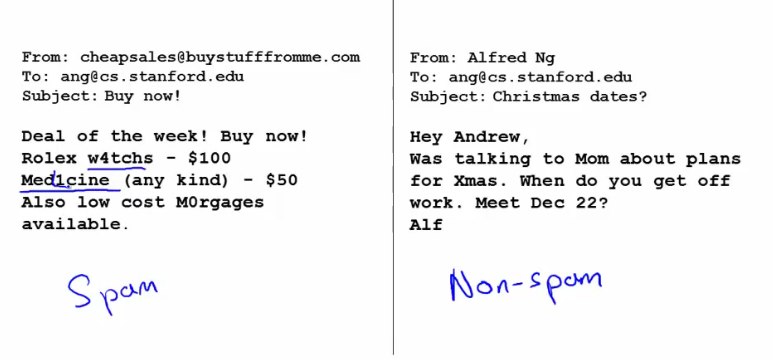
\includegraphics[width=\textwidth]{resources/spam}

\subsection*{Select your own features}
\begin{itemize}
  \item Choose 100 words that indicate if an email is spam or not.
  \item Buy, discount, and deal are examples of spam.
  \item Andrew and now are examples of non-spam.
  \item All these words go into one long vector.
  \item If a matching word does not appear in the email, store 0 in the vector; otherwise, store 1.
  \item Check which word category has the most occurrences.
\end{itemize}

\subsection*{How to improve system accuracy?}
\begin{itemize}
  \item Collect more data.
  \item Develop sophisticated features based on email routing data.
  \item Create a powerful algorithm for detecting misspellings.
  \item Plot learning curves to see whether extra data, features, and so on will help algorithmic optimization.
\end{itemize}

\section*{Error analysis}

\begin{itemize}
  \item Examine the samples (in the cross validation set) on which your algorithm made errors manually.
  \item Try to figure out why.
  \item For example, you may find out that the most prevalent types of spam emails are pharmaceutical emails and phishing emails.
  \item What features would have helped classify them correctly?
\end{itemize}

\section*{Error metrics for skewed analysis}

\begin{itemize}
  \item Suppose we're attempting to categorize cancer patients.
  \item We have 1\% error. Looks good?
  \item But only 0.5\% of people have cancer.
  \item Now, 1\% error looks very bad!
\end{itemize}

\subsection*{Precision and recall}

\begin{table}[hbt!]
  \centering
  \begin{tabular}{|l|l|l|}
    \hline
    Classification & Guessed & Real \\
    \hline
    True positive  & 1       & 1    \\
    False positive & 1       & 0    \\
    True negative  & 0       & 0    \\
    False negative & 0       & 1    \\
    \hline
  \end{tabular}
\end{table}

\begin{itemize}
  \item Precision: How often does our algorithm cause a false alarm?

        $$\frac{true\ positives}{ true\ positives\ +\ false\ positives}$$

  \item Recall: How sensitive is our algorithm?

        $$\frac{true\ positives}{ true\ positives\ +\ false\ negative}$$
\end{itemize}

\subsection*{Trading off precision and recall}

\begin{itemize}
  \item Trained a logistic regression classifier
        \begin{itemize}
          \item Predict 1 if $h_{\theta}(x) >= 0.5$
          \item Predict 0 if $h_{\theta}(x) < 0.5$
        \end{itemize}
  \item We might change the prediction threshold such that we are more sure that a 1 is a true positive.
        \begin{itemize}
          \item Predict 1 if $h_{\theta}(x) >= 0.8$
          \item Predict 0 if $h_{\theta}(x) < 0.2$
        \end{itemize}

  \item But classifier has lower recall - predict y = 1 for a smaller number of patients.
\end{itemize}

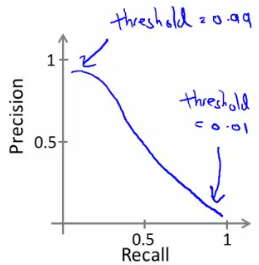
\includegraphics[width=0.4\textwidth]{resources/precission_recall}


~\\
$F_{score}$ is calculated by averaging precision and recall and assigning a larger weight to the lower number.

$$F_{score} = 2 \frac{PR}{P + R}$$

~\\
If you're attempting to establish the threshold automatically, one method is to test a variety of threshold values and assess them on your cross validation set.
Then select the threshold that yields the highest $F_{score}$.

\end{document}
